% Drawing 79/15-7 -- folder 79, batch 15, archive page 285 (PDF page 286).
% Transcription: un carré en pointillés avec ses deux axes et deux diagonales fléchés (les vecteurs $\pm e_1$, $\pm e_2$, $\pm(e_1+e_2)$), étiquetés $s$, $t$, $\lambda^{-1}s$, $\lambda^{-1}t$ ; un hexagone avec trois diagonales formant un triangle inscrit ; un carré ; deux fois $E_0$.
% Kind: dotted square with vectors; hexagon with inscribed triangle; square. Method 2 (schematic redraw from the facsimile). Status: partial.
% Notes: Dotted square with its two axes and two diagonals as arrows from the centre (the vectors +-e1, +-e2, +-(e1+e2)), a heavy point at the left end; a hexagon with three diagonals forming an inscribed triangle; a small square (thick); E_0 twice in the right margin (written sideways). The small labels s, t, lambda^{-1}s, lambda^{-1}t around the dotted square are not legible on the crop and are left out.
% Coordinates: 1 unit = 1 mm = 1/100 of the crop width (bbox in page fractions: [0.5, 0.33, 0.88, 0.56]).
% Redrawn by Claude (claude-opus-5-5), issue #73, 2026-11-07; not checked by a human; not compiled (no TeX in the session).
% Rights: reproduces part of the work -- behind RENDER_TRANSCRIPTS, never published by itself.
\documentclass[tikz,border=3pt]{standalone}
\usepackage{amsmath,amssymb}
\usetikzlibrary{patterns,arrows.meta}
\tikzset{pencil/.style={black!45}, struck/.style={black!35}, mark/.style={circle,draw,inner sep=1.3pt}, pt/.style={circle,fill,inner sep=0.9pt}, opt/.style={circle,draw,fill=white,inner sep=1.1pt}}
\begin{document}
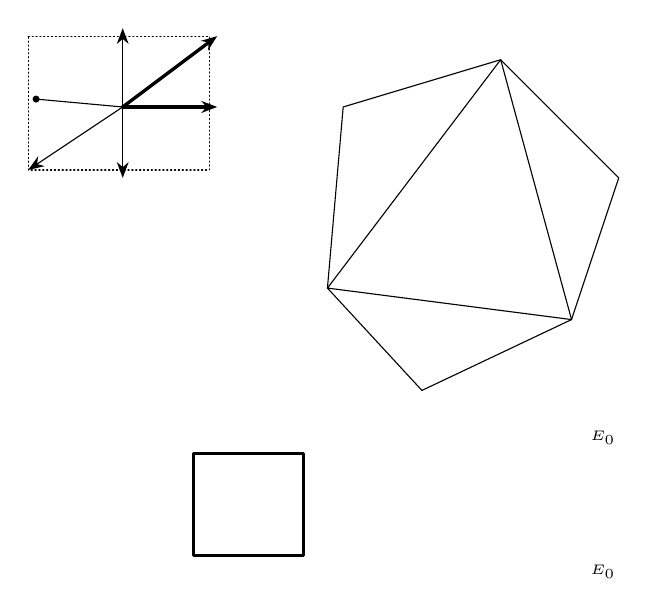
\begin{tikzpicture}[x=1mm,y=1mm,line cap=round,line join=round,font=\scriptsize]
\draw[densely dotted] (20,-15) -- (43,-15) -- (43,-32) -- (20,-32) -- cycle;
\draw[-{Stealth[length=2mm]},very thick] (32,-24) -- (44,-24);
\draw[-{Stealth[length=2mm]}] (32,-24) -- (32,-14);
\draw[-{Stealth[length=2mm]}] (32,-24) -- (32,-33);
\draw (32,-24) -- (21,-23);
\draw[-{Stealth[length=2mm]},very thick] (32,-24) -- (44,-15);
\draw[-{Stealth[length=2mm]}] (32,-24) -- (20,-32);
\node[pt] at (21,-23) {};
\draw (58,-47) -- (60,-24) -- (80,-18) -- (95,-33) -- (89,-51) -- (70,-60) -- cycle;
\draw (58,-47) -- (80,-18) -- (89,-51) -- cycle;
\draw[very thick] (41,-68) -- (55,-68) -- (55,-81) -- (41,-81) -- cycle;
\node[inner sep=1pt] at (93,-66) {\tiny $E_0$};
\node[inner sep=1pt] at (93,-83) {\tiny $E_0$};
\end{tikzpicture}
\end{document}
